\documentclass[UTF8]{ctexart}

\usepackage{subfiles}  

%下面的语句, 引入你的头部设置文件
\usepackage{C:/phpStorm_proj/02_myself_ID_EGO/+100_latex_all_math_sel/myPreamble} 
%必须是绝对路径,才能让各个tex在单独编译时使用到

\title{行列式}


%---------------------------------


\begin{document}
	\tableofcontents % 生成目录
	\date{} % 若不写这句, 则默认也会渲染出日期, 所以我们要手动赋空值
	\maketitle  %这行代码, 让你前面的 title, author, date生效
	
	\section{二阶与三阶行列式}
	
	\subsection{二阶行列式}
	
	$
	\left| \begin{matrix}
		a&		b\\
		c&		d\\
	\end{matrix} \right|=\underset{\text{主对角线}}{\underbrace{ad}}-\underset{\text{副对角线}}{\underbrace{bc}}
	$
	
	
	
		\subsection{三阶行列式}
	$
	\left| \begin{matrix}
		a&		b&		c\\
		d&		e&		f\\
		h&		i&		j\\
	\end{matrix} \right|=\left( aej+bfh+cdi \right) -\left( ceh+dbj+aif \right) 
	$ \\
	
	即: \\
	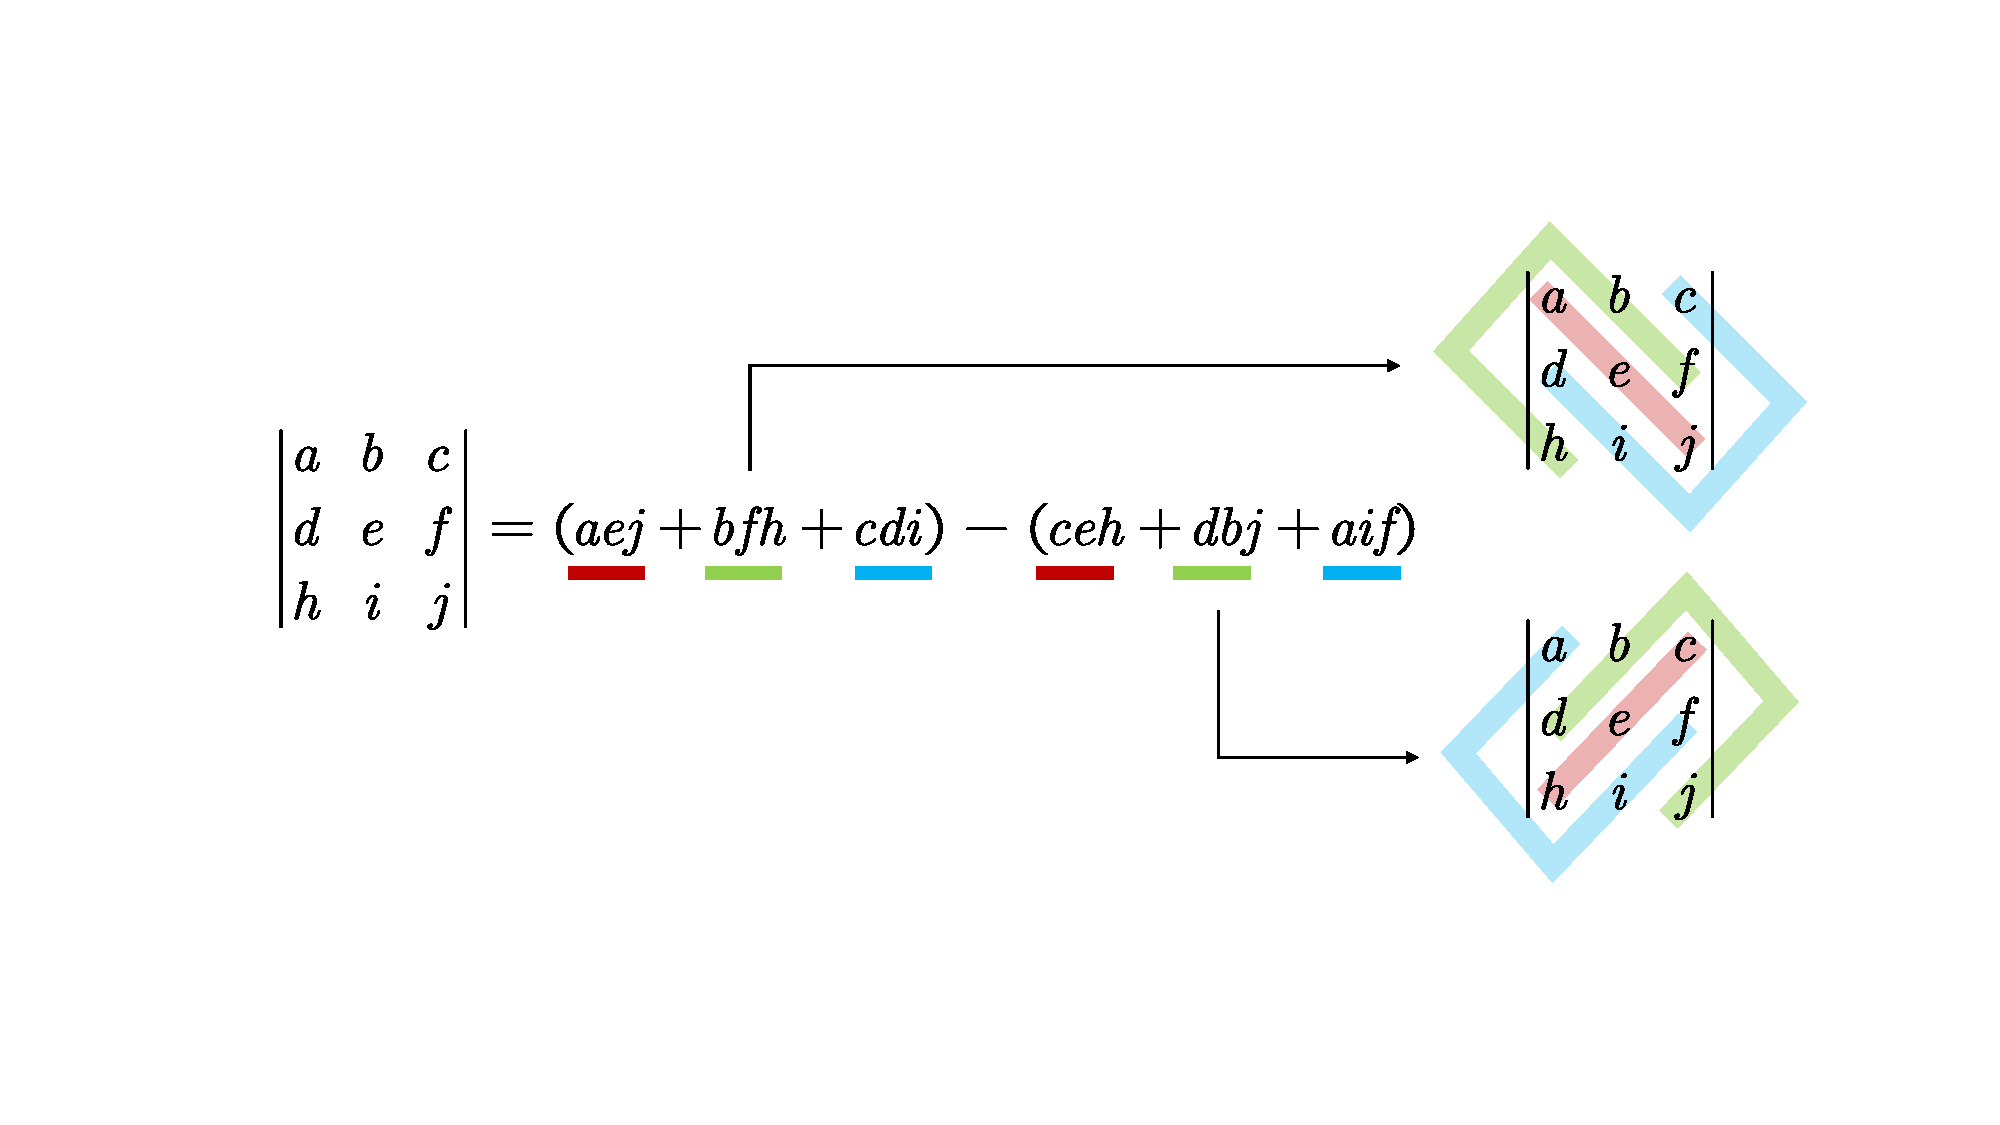
\includegraphics[width=0.8\textwidth]{img/0001.pdf}\\
	
	
	
	
	\section{全排列和对换}
	
	【排列】:\\
	由1,2,...,n 组成的一个``有序"数组, 叫``n级排列".\\
	
	
	
	
	
	
	
	\section{n 阶行列式}
	
	
	\section{行列式的性质}
	
	
	\section{行列式按行(列)展开}
	
	
	
	
	--------------------------------
	
	\section{n阶行列式}
	
	
	\section{行列式的性质}
	
	\subsection{性质1: 行列互换, 其值不变. 即$|A|=\left| A^T \right|$}
	
	\subsection{性质2: 某行(列)元素全为零, 则行列式为零}
	
	\subsection{性质3: 两行(列)元素相等, 或对应成比例, 则行列式为零}
	
	\subsection{性质4: 某行(列)元素均是两个元素之和, 则可拆成两个行列式之和}
	
	\subsection{性质5: 两行(列)互换,行列式的值反号}
	
	\subsection{性质6: 某行(列)元素有公因子$k\left( k\ne 0 \right) $, 则k可提到行列式外面去 }
	
	\subsection{性质7: 某行(列)的b, 倍加到另一行(列)上去, 行列式的值不变 }
	
	
	\section{行列式的展开定理}
	
	\subsection{余子式 $M_{ij}$}
	
	\subsection{代数余子式 $	A_{ij}=\left( -1 \right) ^{i+j}M_{ij}$}
	
	\subsection{按某一行(列)展开的展开公式: \\ $|A|=\sum_{i=1}^n{a_{ij}A_{ij}\ \left( j=1,2,...,n \right)}=\sum_{j=1}^n{a_{ij}A_{ij}\ \left( i=1,2,...,n \right)}$	}
	
	
	
	\section{具体型行列式的计算: $a_{ij}$ 已给出}
	
	\subsection{化为``12+1"型行列式}
	
		\subsubsection{主对角线行列式}
		
		\subsubsection{副对角线行列式}
		
		\subsubsection{拉普拉斯展开式}
		
		\subsubsection{范德蒙德行列式}
	
	\subsection{加边法}
	
	\subsection{递推法 (高阶 → 低阶)}
	
		\subsubsection{建立递推公式,即建立$D_n$ 与 $D_{n-1}$ 的关系}
		
		\subsubsection{$D_n$ 与 $D_{n-1}$ 要有完全相同的元素分布规律, 只是$D_{n-1}$比$D_n$低了一阶 }
	
	
	\subsection{数学归纳 (低阶 → 高阶)}
	
		\subsubsection{第一数学归纳法}
		
		\subsubsection{第二数学归纳法}
	
	
	\section{抽象型行列式的计算: $a_{ij}$ 未给出	}
	
		\subsection{用行列式性质}
		
		\subsection{用矩阵知识}
		
			\subsubsection{设 C=AB, A,B为同阶方阵, 则 $|C|=|AB|=|A||B|$}
			
			\subsubsection{设 C=A+B, A,B为同阶方阵, 则 $|C|=|A+B|$,作恒等变形,转化为矩阵乘积的行列式 }
			
			\subsubsection{设A 为n阶方阵, 则 $|A^*|=|A|^{n-1},\ |(A^*)^*|=\left| \left| A \right|^{n-2}A \right|=\left| A \right|^{\left( n-1 \right) ^2}	$}
		
		\subsection{用相似理论}
		
			\subsubsection{$\left| A \right|=\prod_{i=1}^n{\lambda _i}$}
			
			\subsubsection{若A相似于B, 则 |A|=|B|}
	
	
	
\end{document}